\documentclass[aspectratio=169,11pt]{beamer}
% ==========================================================================
%  KSA lecture-slide theme  =  stock beamer "Boadilla"  +  KSA colour theme
%  brand colours sampled from the official KSA symbol mark:
%    Deep Prussian Blue  #2E3192   (지성 - intellect)
%    Golden Gray         #D6CBB1   (감성 - sensibility)
%  Engine: XeLaTeX.  Usage:
%    \documentclass[aspectratio=169,11pt]{beamer}
%    \input{../../theme/ksa-theme.tex}
%  Each deck lives in its own slides/kor/<deck>/ folder together with its
%  own images; ../../figs/ is kept only as a fallback for the shared cache.
% ==========================================================================

\usepackage{fontspec}
\usepackage{amsmath,amssymb}
\usepackage{graphicx}
\graphicspath{{figs/}{./}{../../../figs/}}
\usepackage{booktabs}
\usepackage{listings}
\usepackage{varwidth}

% ---- fonts (no ctex/xeCJK on this box -> fontspec drives CJK directly) -----
\defaultfontfeatures{Ligatures=TeX}
\setmainfont{Noto Sans CJK KR}
\setsansfont{Noto Sans CJK KR}
\setmonofont{Noto Sans Mono CJK KR}[Scale=0.92]

% ---- base theme: stock Boadilla ------------------------------------------
\usetheme{Boadilla}
\usefonttheme{professionalfonts}
\setbeamertemplate{navigation symbols}{}

% ---- KSA colour theme (recolour the stock theme) --------------------------
\definecolor{ksablue}{HTML}{2E3192}
\definecolor{ksabluedk}{HTML}{20226A}
\definecolor{ksagold}{HTML}{D6CBB1}
\definecolor{ksagolddk}{HTML}{A9976B}
\definecolor{ksared}{HTML}{C0392B}
\definecolor{ksagray}{HTML}{5B5B5B}

\setbeamercolor{structure}{fg=ksablue}
\setbeamercolor{alerted text}{fg=ksared}

\setbeamercolor{palette primary}{fg=white,           bg=ksablue}
\setbeamercolor{palette secondary}{fg=white,         bg=ksablue!85!black}
\setbeamercolor{palette tertiary}{fg=white,          bg=ksabluedk}
\setbeamercolor{titlelike}{fg=ksablue}
\setbeamercolor{frametitle}{fg=ksablue,bg=}
\setbeamercolor{title}{fg=ksablue}
\setbeamercolor{author}{fg=ksagray}
\setbeamercolor{institute}{fg=ksagray}
\setbeamercolor{block title}{fg=white,bg=ksablue}
\setbeamercolor{block body}{fg=black!85,bg=ksablue!6}
\setbeamercolor{item}{fg=ksablue}
\setbeamercolor{section in toc}{fg=black!85}

\setbeamerfont{frametitle}{series=\bfseries}
\setbeamerfont{title}{series=\bfseries}

% ---- footline:  KSA mark | "Made by ..." | n / N   (matches reference) ----
\newcommand{\ksacredit}{}
\setbeamertemplate{footline}{%
  \hbox{%
    \begin{beamercolorbox}[wd=.18\paperwidth,ht=2.6ex,dp=1.5ex,leftskip=1.1em]{}%
      \raisebox{-0.35ex}{\includegraphics[height=2.0ex]{ksa-logo.png}}%
    \end{beamercolorbox}%
    \begin{beamercolorbox}[wd=.64\paperwidth,ht=2.6ex,dp=1.5ex,center]{}%
      {\scriptsize\color{ksagray}\ksacredit}%
    \end{beamercolorbox}%
    \begin{beamercolorbox}[wd=.18\paperwidth,ht=2.6ex,dp=1.5ex,rightskip=1.1em]{}%
      \hfill{\scriptsize\color{ksablue}\insertframenumber\,/\,\inserttotalframenumber}%
    \end{beamercolorbox}%
  }%
  \vskip2pt
}

% ---- section divider: stock \sectionpage, KSA-coloured -------------------
\setbeamertemplate{section page}{%
  \begingroup\centering
    {\color{ksagolddk}\rule{0.16\paperwidth}{1pt}}\par\vskip1.0em
    {\usebeamerfont{title}\color{ksablue}\insertsectionhead\par}\vskip1.0em
    {\color{ksagolddk}\rule{0.16\paperwidth}{1pt}}\par
  \endgroup
}
\AtBeginSection[]{\begin{frame}[plain,noframenumbering]\vfill\sectionpage\vfill\end{frame}}

% ---- code listings ------------------------------------------------------------
\lstdefinestyle{ksa}{%
  basicstyle=\ttfamily\scriptsize,
  keywordstyle=\color{ksablue}\bfseries,
  commentstyle=\color{ksagray}\itshape,
  stringstyle=\color{ksagolddk},
  numberstyle=\tiny\color{ksagray},
  backgroundcolor=\color{ksablue!6},
  frame=leftline, framerule=1.4pt, rulecolor=\color{ksablue},
  xleftmargin=1em, aboveskip=0.8em, belowskip=0.4em,
  showstringspaces=false, breaklines=true, language=Python,
}
\lstset{style=ksa}

% ---- handy macros -----------------------------------------------------------
\newcommand{\kb}[1]{\textbf{\color{ksablue}#1}}   % blue keyword
\newcommand{\kq}[1]{\textbf{\color{ksared}#1}}    % red key-question

\setbeamerfont{title}{series=\bfseries,size=\fontsize{24}{30}\selectfont}
\setbeamerfont{subtitle}{series=\bfseries,size=\fontsize{14}{18}\selectfont}
\setbeamerfont{author}{size=\normalsize}
\setbeamerfont{institute}{size=\small}
\graphicspath{{figs/}{../../../../assets/}}
\makeatletter
\newcommand{\markpage}[1]{\protected@write\@auxout{}{\string\newlabel{#1}{{\the\c@framenumber}{}}}\hypertarget{#1}{}}
\newcommand{\pref}[1]{\hyperlink{#1}{\textcolor{ksagolddk}{(p.\ref{#1})}}}
\makeatother

\renewcommand{\ksacredit}{Machine Learning 1 \,\textperiodcentered\, BatchNorm}
\title{BatchNorm (배치 정규화)}
\subtitle{층마다 값을 평균 0 · 표준편차 1 로 맞추기}
\author{Machine Learning 1}
\institute{한국과학영재학교 (KSA)}
\date{}
\begin{document}
\begin{frame}[plain,noframenumbering]\titlepage\end{frame}

% --- 오늘의 질문
\begin{frame}{오늘의 질문}
\vfill
\centering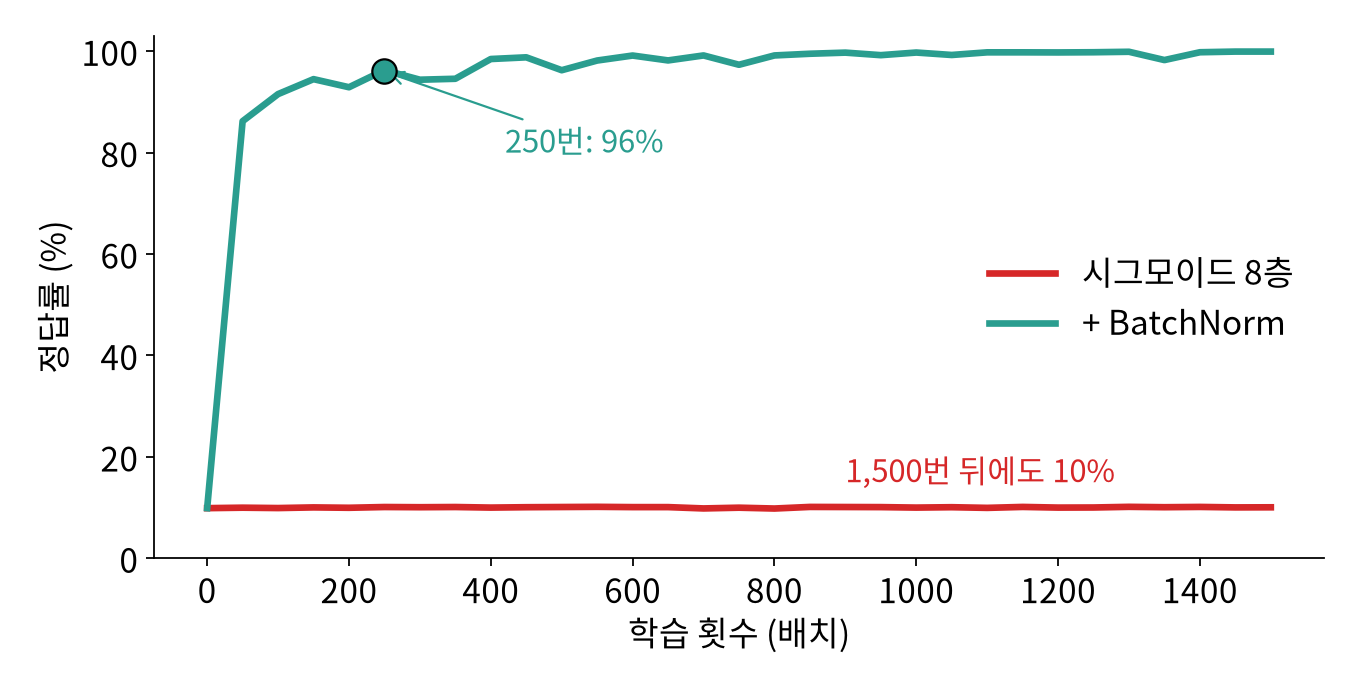
\includegraphics[width=0.6\linewidth]{bn_curve.png}\par\vskip0.2em
{\large 시그모이드 8층: \kq{1,500번 학습해도 10\%} \quad BatchNorm 을 끼우면 \kb{250번에 96\%}}
\vfill
\note{손글씨 숫자를 시그모이드 층 8개짜리 신경망으로 학습했습니다. 1500번을 학습해도 정답률이 10퍼센트, 찍기 수준입니다. 지난 시간의 기울기 소실과 같은 증상입니다. 그런데 층마다 BatchNorm이라는 층을 하나씩 끼워 넣었더니 250번 만에 96퍼센트가 됐습니다. 활성 함수도 가중치 수도 그대로입니다. 오늘은 이 층이 무엇을 하는지 배웁니다.}
\end{frame}

% --- 무슨 일
\begin{frame}{무슨 일이 일어났나: 층을 지날수록 그림들이 똑같아진다}
\markpage{spread}
\vfill
\centering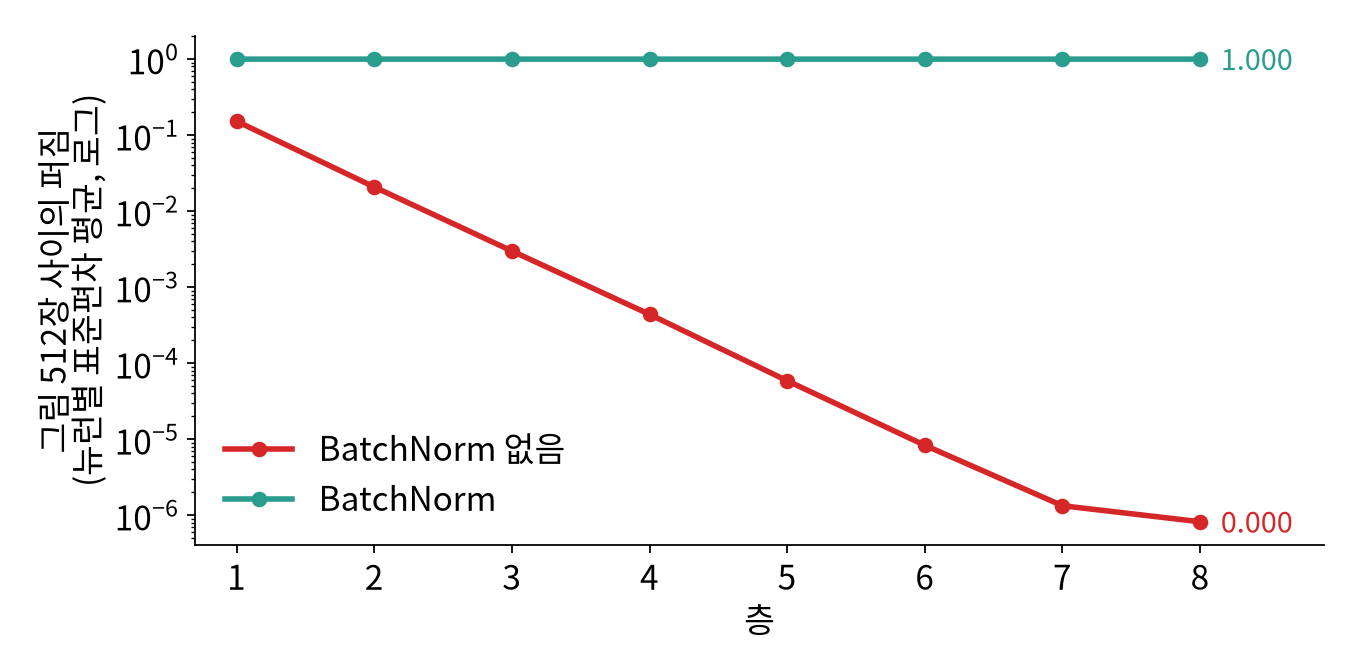
\includegraphics[width=0.58\linewidth]{bn_dist.png}\par\vskip0.2em
{\large 그림 512장이 받는 값의 퍼짐 (학습 전): \quad 1층 0.15 $\to$ 8층 \kq{0.0000002}}\\[0.2em]
{\small 8층에는 모든 그림이 거의 같은 값 $\to$ 구별할 정보가 없다 \quad BatchNorm: 층마다 다시 1 로}
\vfill
\note{BatchNorm이 없을 때 무슨 일이 일어나는지 봅니다. 학습 전에 서로 다른 그림 512장을 넣고, 각 층에서 그림마다 받는 값이 얼마나 다른지, 즉 그림 사이의 퍼짐을 쟀습니다. 1층에서는 0.15인데, 층을 지날 때마다 약 7분의 1로 줄어 8층에서는 0.0000002입니다. 시그모이드가 값을 0.5 근처로 눌러 버리기 때문입니다. 8번째 층 입장에서는 숫자 0 그림이든 9 그림이든 거의 같은 값이 들어오니 구별할 방법이 없고, 기울기도 사라집니다. BatchNorm을 넣으면 층마다 퍼짐을 다시 1로 맞춰 줍니다.}
\end{frame}

% --- 식
\begin{frame}{BatchNorm: 미니배치마다 평균 0, 표준편차 1 로}
\markpage{formula}
\vfill
\centering
{\Large\[ \mu_B = \frac{1}{m}\sum_{i=1}^{m} x_i \qquad \sigma_B^2 = \frac{1}{m}\sum_{i=1}^{m}(x_i - \mu_B)^2 \]}
{\LARGE\[ \hat{x}_i = \frac{x_i - \mu_B}{\sqrt{\sigma_B^2 + \epsilon}} \qquad y_i = \textcolor{ksablue}{\gamma}\,\hat{x}_i + \textcolor{ksared}{\beta} \]}\vskip0.3em
\renewcommand{\arraystretch}{1.25}
{\normalsize\begin{tabular}{ll}
$m$ & 미니배치 크기 \quad 뉴런마다 따로 계산한다\\
$\epsilon$ & 0 으로 나누지 않게 더하는 아주 작은 수 (예: $10^{-5}$)\\
\textcolor{ksablue}{$\gamma$}, \textcolor{ksared}{$\beta$} & \textbf{학습하는} 크기 · 위치 (처음엔 1, 0)
\end{tabular}}
\vfill
\note{BatchNorm이 하는 일입니다. 뉴런 하나가 미니배치의 데이터 m개에게서 받은 값들로 평균과 분산을 구합니다. 각 값에서 평균을 빼고 표준편차로 나누면 평균 0, 표준편차 1이 됩니다. 가우시안 시간의 z 점수와 같은 식입니다. 엡실론은 분산이 0일 때 0으로 나누지 않게 더하는 아주 작은 수입니다. 그다음 감마를 곱하고 베타를 더합니다. 감마와 베타는 가중치처럼 역전파로 학습하는 숫자이고, 처음에는 1과 0으로 시작합니다. 이 계산은 뉴런마다 따로 합니다.}
\end{frame}

% --- 손 계산
\begin{frame}{손으로 한 번}
\vfill
\centering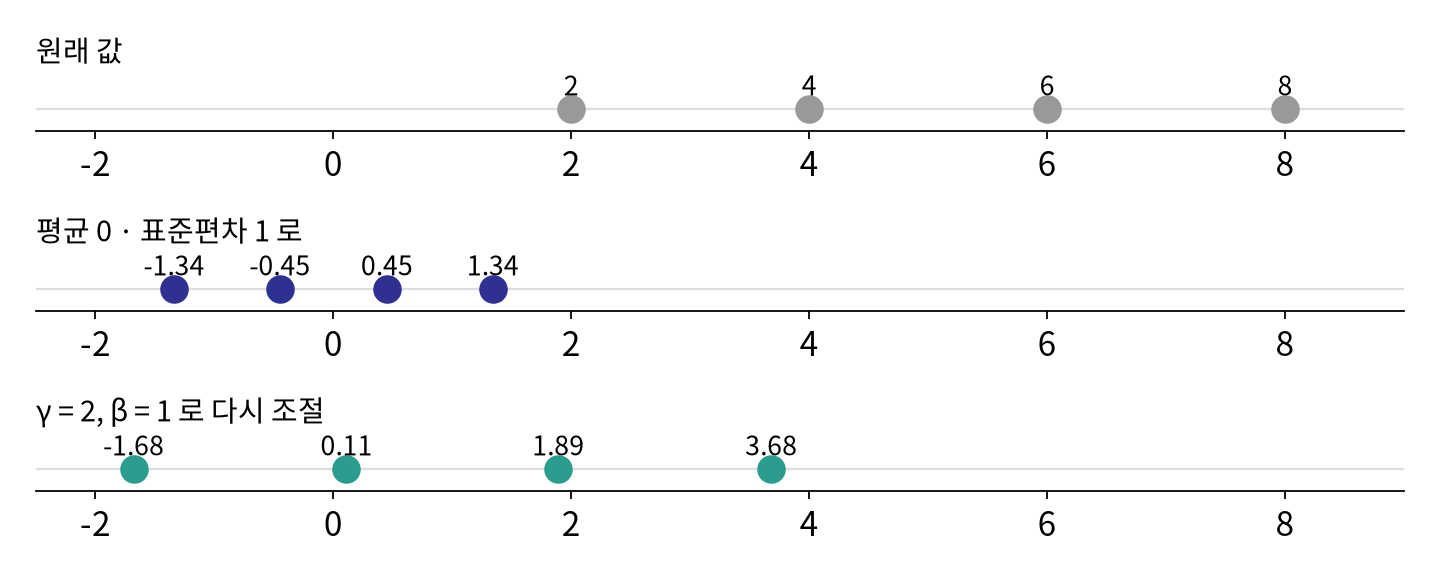
\includegraphics[width=0.66\linewidth]{bn_hand.png}\par\vskip0.2em
{\large 배치 4개에서 받은 값 2, 4, 6, 8 \quad $\mu_B = 5$, \; $\sigma_B^2 = \frac{9 + 1 + 1 + 9}{4} = 5$}\\[0.3em]
{\large $\hat{x} = \frac{x - 5}{\sqrt5}$: $-1.34, -0.45, 0.45, 1.34$ \quad $\gamma = 2, \beta = 1$: \; $-1.68, 0.11, 1.89, 3.68$}
\vfill
\note{작은 예로 해 봅니다. 뉴런 하나가 배치 4개에서 2, 4, 6, 8을 받았습니다. 평균은 5, 평균에서 떨어진 거리의 제곱은 9, 1, 1, 9라서 분산은 5입니다. 평균을 빼고 루트 5로 나누면 마이너스 1.34, 마이너스 0.45, 0.45, 1.34가 됩니다. 평균 0, 표준편차 1입니다. 학습된 감마가 2, 베타가 1이라면 2를 곱하고 1을 더해 마이너스 1.68, 0.11, 1.89, 3.68을 다음 층으로 보냅니다.}
\end{frame}

% --- 감마 베타
\begin{frame}{왜 $\gamma$, $\beta$ 를 다시 곱하고 더하나}
\vfill
\centering
{\large 항상 평균 0 · 표준편차 1 로 묶어 두면 \quad 시그모이드의 \textbf{가운데 직선 부분}만 쓰게 된다}\\[0.8em]
{\large $\gamma, \beta$ 를 학습하면 신경망이 \kb{알맞은 크기와 위치를 스스로} 고른다}\\[0.8em]
{\Large 필요하면 \; $\gamma = \sigma_B$, \; $\beta = \mu_B$ \; $\to$ \; \textbf{원래 값으로 되돌릴 수도} 있다}\\[0.8em]
{\small 그래서 BatchNorm 을 넣어도 신경망이 표현할 수 있는 것은 줄어들지 않는다}
\vfill
\note{정규화만 하면 되는데 왜 감마와 베타를 다시 곱하고 더할까요? 모든 층의 값을 항상 평균 0, 표준편차 1로 묶어 두면, 시그모이드에서는 0 근처의 거의 직선인 부분만 쓰게 되어 비선형성을 제대로 활용하지 못할 수 있습니다. 감마와 베타를 학습하게 하면 신경망이 층마다 알맞은 크기와 위치를 스스로 고릅니다. 극단적으로 감마를 원래 표준편차, 베타를 원래 평균으로 학습하면 정규화 전의 값으로 되돌릴 수도 있습니다. 그러니 BatchNorm을 넣어서 신경망이 표현할 수 있는 것이 줄어들지는 않습니다.}
\end{frame}

% --- 결과
\begin{frame}{효과}
\vfill
\centering
\renewcommand{\arraystretch}{1.5}
{\large\begin{tabular}{ll}
우리 실험 (시그모이드 8층) & \kq{10\%} $\to$ 250번에 \kb{96\%}\\
논문 (2015, ImageNet) & 같은 정확도를 \kb{14배 적은} 학습으로\\
덤 & 큰 학습률도 안정 · 초기화에 덜 민감 · 약간의 정규화
\end{tabular}}\vskip0.8em
{\small 왜 잘 되는지: 처음엔 ``층 입력 분포의 출렁임 (internal covariate shift) 을 줄인다''고 설명했지만,\\ 지금은 ``손실 지형을 매끄럽게 만들어 큰 걸음을 가능하게 한다''는 설명이 더 받아들여진다}
\vfill
\note{효과를 정리합니다. 우리 실험에서는 1500번에 10퍼센트였던 신경망이 250번에 96퍼센트가 됐습니다. 2015년 구글의 이오페와 세게디의 논문에서는 이미지넷에서 같은 정확도를 14배 적은 학습으로 얻었습니다. 덤으로 학습률을 크게 잡아도 안정적이고, 초기화를 덜 신경 써도 되고, 미니배치마다 평균이 조금씩 흔들리는 것이 약간의 정규화 효과도 줍니다. 왜 잘 되는지에 대해서는 논쟁이 있습니다. 논문은 층 입력 분포의 출렁임을 줄인다고 설명했지만, 이후 연구에서는 손실 지형을 매끄럽게 만들어 큰 걸음으로도 안정적으로 내려갈 수 있게 한다는 설명이 더 받아들여지고 있습니다.}
\end{frame}

% --- 시험 때
\begin{frame}{시험 때는 모아 둔 평균을 쓴다}
\markpage{eval}
\vfill
\centering
{\large 시험 때는 그림이 \textbf{한 장씩} 들어올 수도 있다 $\to$ 배치 평균을 구할 수 없다}\vskip0.6em
{\Large\[ \mu_{\text{run}} \leftarrow 0.9\,\mu_{\text{run}} + 0.1\,\mu_B \qquad \sigma^2_{\text{run}} \leftarrow 0.9\,\sigma^2_{\text{run}} + 0.1\,\sigma_B^2 \]}\vskip0.3em
{\large 학습하면서 배치 평균 · 분산을 \textbf{조금씩 모아} 두었다가 시험 때 그 값을 쓴다}\\[0.6em]
{\large \texttt{model.train()} = 배치 통계 \quad \texttt{model.eval()} = \kb{모아 둔 통계}}
\vfill
\note{시험할 때는 문제가 하나 있습니다. 그림이 한 장씩 들어올 수도 있어서 배치 평균을 구할 수 없습니다. 한 장이면 평균을 빼면 항상 0이 되니까요. 그래서 학습하는 동안 배치 평균과 분산을 조금씩 모아 둡니다. 이전 값의 0.9와 이번 배치 값의 0.1을 섞는 식으로 계속 갱신합니다. 시험 때는 이 모아 둔 평균과 분산으로 정규화합니다. PyTorch에서는 드롭아웃과 같은 스위치입니다. train 모드에서는 배치 통계를, eval 모드에서는 모아 둔 통계를 씁니다. eval을 깜빡하면 시험 결과가 배치 구성에 따라 달라집니다.}
\end{frame}

% --- 어디에
\begin{frame}{어디에 넣나, 그리고 친척들}
\vfill
\centering
\renewcommand{\arraystretch}{1.5}
{\large\begin{tabular}{ll}
위치 & \texttt{Linear} (합성곱) $\to$ \textbf{BatchNorm} $\to$ 활성 함수\\
합성곱 (10주차) & 채널마다 평균 · 분산 (\texttt{BatchNorm2d}) \quad ResNet 의 기본 부품\\
\kq{약점} & 배치가 작으면 평균이 불안정, 순서 데이터에 어색\\
\textbf{LayerNorm} & \textbf{한 데이터 안의} 뉴런들로 평균 · 분산 (트랜스포머)
\end{tabular}}
\vfill
\note{어디에 넣을까요? 원 논문은 Linear 층이나 합성곱 층 다음, 활성 함수 앞에 넣었습니다. 10주차 합성곱 신경망에서는 채널마다 평균과 분산을 구하는 BatchNorm2d를 쓰고, ResNet의 기본 부품입니다. 약점도 있습니다. 배치가 2개처럼 아주 작으면 배치 평균이 너무 흔들리고, 문장처럼 길이가 다른 순서 데이터에는 어색합니다. 그래서 배치 대신 데이터 하나 안의 뉴런들로 평균과 분산을 구하는 LayerNorm이 나왔고, 12주차 트랜스포머는 LayerNorm을 씁니다.}
\end{frame}

% --- 문제풀이
\begin{frame}{문제풀이}
\vfill
\begin{enumerate}
\item 배치 값 1, 3, 5, 7 을 BatchNorm 하면? ($\epsilon$ 무시, $\gamma = 1$, $\beta = 0$)\vskip0.8em
\item 위에서 $\gamma = 3$, $\beta = 10$ 이면 출력의 평균과 표준편차는?\vskip0.8em
\item 학습이 끝난 모델로 그림 한 장을 예측했더니 이상한 답이 나왔다. \texttt{model.train()} 상태였다. 왜 문제인가?\vskip0.8em
\item 배치 크기 1 로 학습하면 BatchNorm 은 어떻게 되나?
\end{enumerate}
\vfill
\note{1번 답. 평균 4, 거리 제곱 9, 1, 1, 9로 분산 5, 표준편차 루트 5입니다. 마이너스 1.34, 마이너스 0.45, 0.45, 1.34입니다. 2번 답. 평균 10, 표준편차 3입니다. 3번 답. 그림 한 장으로 배치 평균을 구하니 정규화하면 모든 값이 0이 되어 버립니다. eval 모드로 모아 둔 통계를 써야 합니다. 4번 답. 평균이 자기 자신이라 정규화한 값이 항상 0이고 분산도 0이라 학습이 안 됩니다. 실제로 PyTorch는 오류를 냅니다.}
\end{frame}

% --- 실습
\begin{frame}{실습}
\vfill
\centering\begin{tabular}{rl}
\large 1 & BatchNorm 직접 구현 $\to$ 2, 4, 6, 8 손 계산 재현, \texttt{nn.BatchNorm1d} 와 비교\\[0.5em]
\large 2 & 시그모이드 8층: 층별 퍼짐과 학습 곡선, BatchNorm 있음 vs 없음\\[0.5em]
\large 3 & \texttt{train()} / \texttt{eval()}: 그림 한 장 예측과 모아 둔 평균 (\texttt{running\_mean})
\end{tabular}\vskip1em
Optical Recognition of Handwritten Digits (UCI; scikit-learn \texttt{load\_digits}) \\[0.4em]\href{https://colab.research.google.com/github/SuminHan/book-ml/blob/main/slides/v2/ml1/week09/batchnorm/lab/batchnorm.ipynb}{\textcolor{ksagolddk}{▶ Colab에서 실습 노트북 열기}}
\vfill
\note{실습은 세 부분입니다. 첫째, BatchNorm을 직접 구현해서 손 계산을 재현하고 PyTorch의 BatchNorm1d와 비교합니다. 둘째, 시그모이드 8층 신경망에서 층별 퍼짐과 학습 곡선을 BatchNorm이 있을 때와 없을 때 비교합니다. 셋째, train과 eval 모드에서 그림 한 장을 예측해 보고, 모아 둔 평균이 어떻게 쓰이는지 확인합니다.}
\end{frame}

% --- 정리
\begin{frame}{정리}
\vfill
\centering\large\begin{tabular}{l}
깊은 시그모이드: 층을 지날수록 그림들이 같은 값이 된다 (0.15 $\to$ 0.0000002)\\[0.5em]
\textbf{BatchNorm} \quad 미니배치마다 뉴런별 평균 0 · 표준편차 1, 그다음 $\gamma \hat{x} + \beta$\\[0.5em]
10\% $\to$ 250번에 96\% \quad 논문: 14배 적은 학습 \quad 큰 학습률도 안정\\[0.5em]
시험 때는 모아 둔 평균 · 분산 (\texttt{eval()}) \quad 트랜스포머는 LayerNorm
\end{tabular}
\vfill
\note{정리합니다. 깊은 시그모이드 신경망에서는 층을 지날수록 서로 다른 그림들이 거의 같은 값을 받게 되어 학습이 멈춥니다. BatchNorm은 미니배치마다 뉴런별로 평균 0, 표준편차 1로 맞춘 뒤 학습하는 감마와 베타로 크기와 위치를 다시 조절합니다. 우리 실험에서 10퍼센트가 250번 만에 96퍼센트가 됐고, 논문에서는 14배 적은 학습으로 같은 정확도를 얻었습니다. 시험 때는 학습 중에 모아 둔 평균과 분산을 쓰고, 트랜스포머는 그 친척인 LayerNorm을 씁니다.}
\end{frame}
\end{document}
